%Version 31 December 2024
% See section 11 of the User Manual for version history
%
%%%%%%%%%%%%%%%%%%%%%%%%%%%%%%%%%%%%%%%%%%%%%%%%%%%%%%%%%%%%%%%%%%%%%%
%%                                                                 %%
%% Please do not use \input{...} to include other tex files.       %%
%% Submit your LaTeX manuscript as one .tex document.              %%
%%                                                                 %%
%% All additional figures and files should be attached             %%
%% separately and not embedded in the \TeX\ document itself.       %%
%%                                                                 %%
%%%%%%%%%%%%%%%%%%%%%%%%%%%%%%%%%%%%%%%%%%%%%%%%%%%%%%%%%%%%%%%%%%%%%

%%\documentclass[referee,sn-basic]{sn-jnl}% referee option is meant for double line spacing

%%=======================================================%%
%% to print line numbers in the margin use lineno option %%
%%=======================================================%%

%%\documentclass[lineno,sn-basic]{sn-jnl}% Basic Springer Nature Reference Style/Chemistry Reference Style

%%======================================================%%
%% to compile with pdflatex/xelatex use pdflatex option %%
%%======================================================%%

%%\documentclass[pdflatex,sn-basic]{sn-jnl}% Basic Springer Nature Reference Style/Chemistry Reference Style


%%Note: the following reference styles support Namedate and Numbered referencing. By default the style follows the most common style. To switch between the options you can add or remove “Numbered” in the optional parenthesis. 
%%The option is available for: sn-basic.bst, sn-vancouver.bst, sn-chicago.bst%  
 
%%\documentclass[pdflatex,sn-nature]{sn-jnl}% Style for submissions to Nature Portfolio journals
%%\documentclass[pdflatex,sn-basic]{sn-jnl}% Basic Springer Nature Reference Style/Chemistry Reference Style
\documentclass[pdflatex,sn-mathphys-num]{sn-jnl}% Math and Physical Sciences Numbered Reference Style 
%%\documentclass[pdflatex,sn-mathphys-ay]{sn-jnl}% Math and Physical Sciences Author Year Reference Style
%%\documentclass[pdflatex,sn-aps]{sn-jnl}% American Physical Society (APS) Reference Style
%%\documentclass[pdflatex,sn-vancouver,Numbered]{sn-jnl}% Vancouver Reference Style
%%\documentclass[pdflatex,sn-apa]{sn-jnl}% APA Reference Style 
%%\documentclass[pdflatex,sn-chicago]{sn-jnl}% Chicago-based Humanities Reference Style

%%%% Standard Packages
%%<additional latex packages if required can be included here>

\usepackage{graphicx}%
\usepackage{multirow}%
\usepackage{amsmath,amssymb,amsfonts}%
\usepackage{amsthm}%
\usepackage{mathrsfs}%
\usepackage[title]{appendix}%
% \usepackage{xcolor}%
\usepackage{textcomp}%
\usepackage{manyfoot}%
\usepackage{booktabs}%
\usepackage{algorithm}%
\usepackage{algorithmicx}%
\usepackage{algpseudocode}%
\usepackage{listings}%
%%%%

\usepackage[utf8]{inputenc}  % Dùng mã hóa UTF-8
\usepackage[T5]{fontenc}     % Chọn bộ mã T5 cho tiếng Việt
\usepackage[english]{babel} 
\usepackage{titlesec}

\usepackage{graphicx} % Để chèn hình ảnh
\usepackage{caption}  % Để căn chỉnh caption
\captionsetup[figure]{justification=centering} 
\usepackage{subcaption}

\usepackage[
backend=biber,
style=numeric,
sorting=ynt
]{biblatex}

\addbibresource{sn-bibliography.bib}

%%%%%=============================================================================%%%%
%%%%  Remarks: This template is provided to aid authors with the preparation
%%%%  of original research articles intended for submission to journals published 
%%%%  by Springer Nature. The guidance has been prepared in partnership with 
%%%%  production teams to conform to Springer Nature technical requirements. 
%%%%  Editorial and presentation requirements differ among journal portfolios and 
%%%%  research disciplines. You may find sections in this template are irrelevant 
%%%%  to your work and are empowered to omit any such section if allowed by the 
%%%%  journal you intend to submit to. The submission guidelines and policies 
%%%%  of the journal take precedence. A detailed User Manual is available in the 
%%%%  template package for technical guidance.
%%%%%=============================================================================%%%%

%% as per the requirement new theorem styles can be included as shown below
\theoremstyle{thmstyleone}%
\newtheorem{theorem}{Theorem}%  meant for continuous numbers
%%\newtheorem{theorem}{Theorem}[section]% meant for sectionwise numbers
%% optional argument [theorem] produces theorem numbering sequence instead of independent numbers for Proposition
\newtheorem{proposition}[theorem]{Proposition}% 
%%\newtheorem{proposition}{Proposition}% to get separate numbers for theorem and proposition etc.

\theoremstyle{thmstyletwo}%
\newtheorem{example}{Example}%
\newtheorem{remark}{Remark}%

\theoremstyle{thmstylethree}%
\newtheorem{definition}{Definition}%

\raggedbottom
%%\unnumbered% uncomment this for unnumbered level heads

\begin{document}

\title[Article Title]{The effectiveness of channel and spatial attention for improving image classification}

%%=============================================================%%
%% GivenName	-> \fnm{Joergen W.}
%% Particle	-> \spfx{van der} -> surname prefix
%% FamilyName	-> \sur{Ploeg}
%% Suffix	-> \sfx{IV}
%% \author*[1,2]{\fnm{Joergen W.} \spfx{van der} \sur{Ploeg} 
%%  \sfx{IV}}\email{iauthor@gmail.com}
%%=============================================================%%

\author{\fnm{Le Thao Tram}\sur{Nguyen}}
\author{\fnm{Minh Phung} \sur{Bui}}
\author[*]{\fnm{Quoc Huy} \sur{Nguyen}}


\affil{\orgdiv{Saigon University}, \country{VietNam}}

\affil[*]{Corresponding author: nqhuy@sgu.edu.vn}



%%==================================%%
%% Sample for unstructured abstract %%
%%==================================%%
\abstract{Image classification has witnessed remarkable progress due to the advent of Convolutional Neural Networks  (CNNs). However, the capacity to focus on salient information within images remains a challenge. This research explores the integration of Channel Attention and Spatial Attention mechanisms into baseline CNN architectures to enhance classification performance. We conduct experiments on standard image classification datasets to evaluate the efficacy of integrating CBAM \cite{b7} (Convolutional Block Attention Module), BAM \cite{b8} (Bottleneck Attention Module), and scSE \cite{b9} (spatial and channel Squeeze \& Excitation) against baseline models. Experimental results demonstrate that leveraging these attention modules significantly improves classification accuracy.}

%%================================%%
%% Sample for structured abstract %%
%%================================%%

% \abstract{\textbf{Purpose:} The abstract serves both as a general introduction to the topic and as a brief, non-technical summary of the main results and their implications. The abstract must not include subheadings (unless expressly permitted in the journal's Instructions to Authors), equations or citations. As a guide the abstract should not exceed 200 words. Most journals do not set a hard limit however authors are advised to check the author instructions for the journal they are submitting to.
% 
% \textbf{Methods:} The abstract serves both as a general introduction to the topic and as a brief, non-technical summary of the main results and their implications. The abstract must not include subheadings (unless expressly permitted in the journal's Instructions to Authors), equations or citations. As a guide the abstract should not exceed 200 words. Most journals do not set a hard limit however authors are advised to check the author instructions for the journal they are submitting to.
% 
% \textbf{Results:} The abstract serves both as a general introduction to the topic and as a brief, non-technical summary of the main results and their implications. The abstract must not include subheadings (unless expressly permitted in the journal's Instructions to Authors), equations or citations. As a guide the abstract should not exceed 200 words. Most journals do not set a hard limit however authors are advised to check the author instructions for the journal they are submitting to.
% 
% \textbf{Conclusion:} The abstract serves both as a general introduction to the topic and as a brief, non-technical summary of the main results and their implications. The abstract must not include subheadings (unless expressly permitted in the journal's Instructions to Authors), equations or citations. As a guide the abstract should not exceed 200 words. Most journals do not set a hard limit however authors are advised to check the author instructions for the journal they are submitting to.}

\keywords{Image classification; Deep learning; Attention mechanism; Channel Attention; Spatial Attention}

%%\pacs[JEL Classification]{D8, H51}

%%\pacs[MSC Classification]{35A01, 65L10, 65L12, 65L20, 65L70}

\maketitle

\section{Introduction}\label{sec1}
%% Text of abstract
The rapid advancements in deep learning have revolutionized image classification, with Convolutional Neural Networks (CNNs) emerging as a dominant paradigm due to their efficacy in extracting hierarchical feature representations. Despite the success of these architectures, challenges persist in enhancing their capacity to focus on pertinent information within images, particularly in scenarios demanding discrimination between intricate data patterns.
To mitigate this limitation, attention mechanisms have garnered significant attention as a potent means of boosting model performance by dynamically emphasizing salient features. Among the diverse array of attention mechanisms, Channel Attention and Spatial Attention have demonstrated considerable potential\cite{b1}. Channel Attention prioritizes informative feature maps by adaptively assigning weights, thereby enabling the model to accentuate features exhibiting higher relevance\cite{b4}. Conversely, Spatial Attention concentrates on the spatial localities of the input image, highlighting crucial regions while suppressing less pertinent ones\cite{b4}. The synergistic integration of these two mechanisms presents a promising avenue for augmenting the discriminative power of image classification models.
This paper investigates the incorporation of Channel Attention and Spatial Attention mechanisms into baseline image classification architectures. By leveraging these mechanisms, we aim to enhance the efficiency and accuracy of feature extraction, consequently improving classification performance. To rigorously evaluate the efficacy of the proposed approach, we conduct extensive experiments comparing established baseline models with their augmented counterparts integrating Channel Attention and Spatial Attention modules.
\begin{figure}[h]
  \centering
  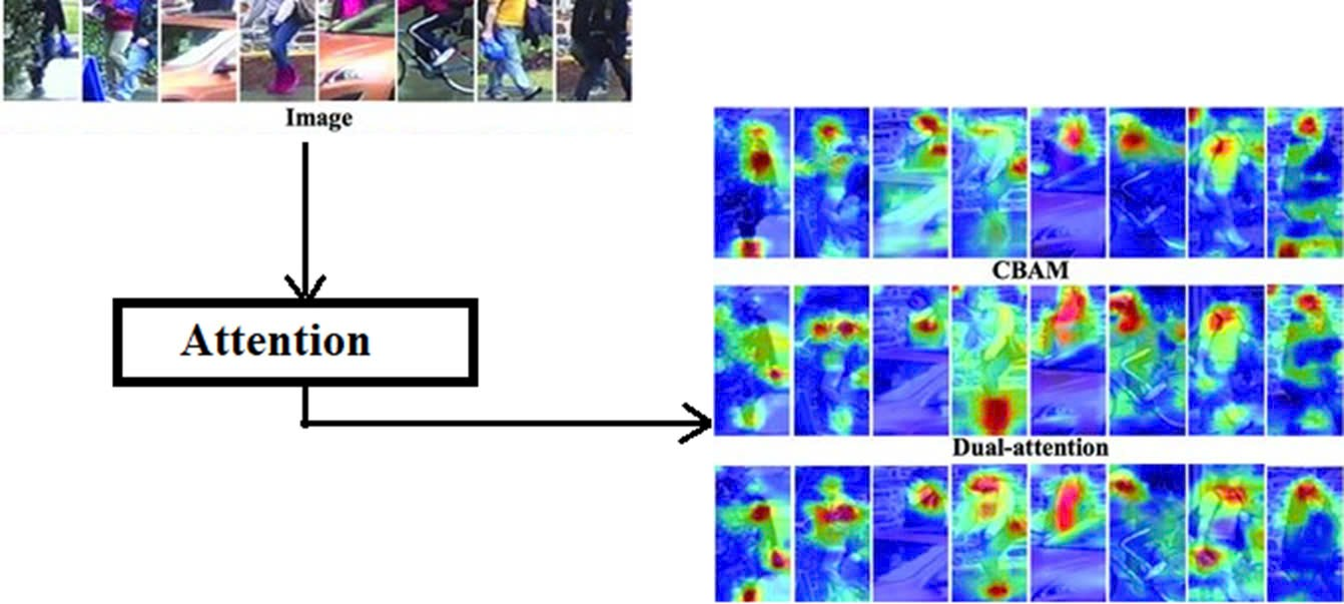
\includegraphics[width=0.8\textwidth]{Figures/intro2.png}
   \caption{The impact of attention mechanisms}
  \label{fig:h1}
\end{figure}



With rapid development, from fundamental concepts to recent breakthroughs, attention mechanisms have been continuously researched and refined. The genesis of attention mechanisms can be traced back to the Recurrent Attention Model (RAM) in 2014. RAM introduced the concept of a sequential attention network, enabling the model to focus on relevant regions within an image using reinforcement learning. However, RAM was limited by its sequential structure, hindering parallel processing capabilities. Subsequently, Spatial Transformer Networks (STN) in 2015 augmented the ability to perform spatial transformations directly on image data, allowing the network to automatically adjust relevant regions for easier recognition without altering the loss function. In 2018, the Non-local Network \cite{b16} emerged with the goal of modeling complex spatio-temporal relationships within data. Despite achieving high performance, the Non-local Network lacked the capacity to model inter-channel correlations. To address this, variants such as the Compact Generalized Non-local Network were developed, improving the efficiency of processing complex data. In 2019, Expectation-Maximization Attention (EMA) \cite{b17} was proposed with a lightweight structure, easily integrated into CNNs, enhancing efficiency and reducing computational cost. Following this, SENet (Squeeze-and-Excitation Network) \cite{b18} in 2020 focused on inter-channel relationships, recalibrating features to enhance generalization capabilities on large datasets. SENet demonstrated superior performance with a negligible increase in computational overhead. More recently, Vision Transformers (ViTs) \cite{b19} have been successfully applied in image classification, overcoming many limitations of CNNs. However, the performance of ViTs saturates quickly with increasing network depth, leading to the development of DeepViT, an improvement that enhances the diversity of attention maps at low cost. In 2021, Tokens-To-Token Vision Transformer (T2T-ViT) \cite{b20} further enhanced performance by reducing parameters and computational cost, while achieving superior accuracy compared to previous architectures. In 2023, a new advancement was marked by the Distract your Attention Network (DAN) \cite{b21}. DAN combines three main components: a Feature Clustering Network (FCN), a Multi-head Attention Network (MAN), and an Attention Fusion Network (AFN).

\section{Related works}\label{sec2}
\subsection{ResNet}
ResNet (Residual Network) is a deep neural network architecture introduced in 2015 by Kaiming He et al. In traditional neural networks, each layer takes input from the previous layer and passes the output to the next layer. In deep neural networks, the outputs from the early layers can be significantly altered by the time they reach the later layers, making training difficult due to the "vanishing gradient" problem. ResNet has overcome this problem by introducing skip connections. These connections allow information to be directly transmitted from one layer to another without passing through all intermediate layers, helping to maintain gradients and improve training. ResNet is similar to traditional neural networks, consisting of stacked convolutional, pooling, activation, and fully-connected layers, organized into multiple stages, with each stage containing a number of residual blocks with an increasing number of filters. Each stage can reduce the spatial dimension of features and increase the number of feature channels. The specific architecture of a ResNet can vary depending on the number of layers (ResNet-18, ResNet-34, ResNet-50, ResNet-101, ResNet-152).


\begin{figure}[h]
  \centering
  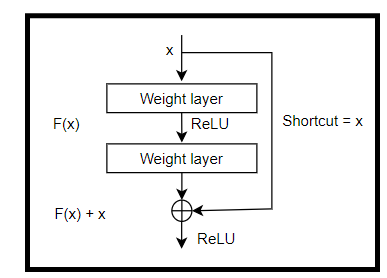
\includegraphics[width=0.3\textwidth]{Figures/residual2.png}
   \caption{Residual block formula}
  \label{fig:h4}
\end{figure}
A residual block is computed as y = F(x) + x, where x is the input to the block, y is the output, and F(x) is a function representing non-linear transformations (such as convolutional layers, batch normalization, and ReLU) applied to x. 

\subsection{VGGNet}
In 2014, Simonyan and Zisserman published the Visual Geometry Group (VGGNet) research, demonstrating that the depth of a Convolutional Neural Network (CNN) could be increased through the use of small-sized filters. The authors showcased significant improvements over previous studies by scaling the network depth to 16–19 layers. Furthermore, they introduced this model with a simple and sequential architecture.

\begin{figure}[h]
  \centering
  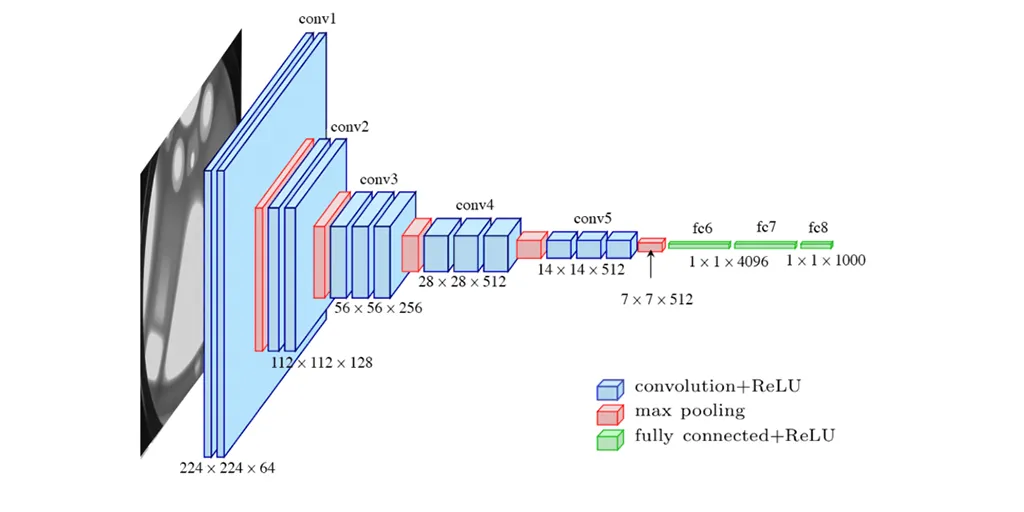
\includegraphics[width=0.9\textwidth]{Figures/vgg.png}
   \caption{VGG-16 Architecture}
  \label{fig:h5}
\end{figure}

\subsection{CBAM - Convolutional Block Attention Module}
To enhance informative channels as well as important regions,
Woo et al. \cite{b7} proposed the convolutional block attention module
(CBAM) which stacks channel attention and spatial attention
in series. It decouples the channel attention map and spatial
attention map for computational efficiency, and leverages
spatial global information by introducing global pooling.

Channel attention module: The Channel Attention Module focuses on learning weights for each feature channel. It assesses the relative importance of each channel and adjusts their intensities. This module concurrently employs both average-pooling and max-pooling operations, as this combined approach can enhance the network's representational capacity compared to using each operation independently. Finally, the output feature vectors are merged using element-wise summation to generate a channel feature map.
% \[
% M_c(X) = \sigma\left(\text{MLP}\left(\text{AvgPool}(X)\right) + \text{MLP}\left(\text{MaxPool}(X)\right)\right)
% \]
\begin{equation}\label{eq:cbam-channel}
M_c(X) = \sigma\bigl(\mathrm{MLP}(\mathrm{AvgPool}(X)) + \mathrm{MLP}(\mathrm{MaxPool}(X))\bigr)
\end{equation}
Spatial attention module: This module focuses on learning weights for each spatial location on the feature map. It assesses the relative importance of different locations and adjusts their intensities. To compute spatial attention, it first performs average-pooling and max-pooling operations along the channel axis and concatenates them to generate an efficient feature descriptor.

% \[
% M_s(X) = \sigma\left(\text{Conv2D}\left(\left[\text{AvgPool}(X), \text{MaxPool}(X)\right]\right)\right)  
% \]
\begin{equation}\label{eq:cbam-spatial}
M_s(X) = \sigma\Bigl(\mathrm{Conv2D}\bigl(\bigl[\mathrm{AvgPool}(X),\,\mathrm{MaxPool}(X)\bigr]\bigr)\Bigr)
\end{equation}
CBAM\cite{b7} combines information from both channel and spatial attention to emphasize the most salient features.
% \[
% X_{\text{out}} = X \odot M_c(X) \odot M_s(X)
% \]
\begin{equation}\label{eq:cbam-out}
X_{\mathrm{out}} = X \odot M_c(X) \odot M_s(X)
\end{equation}
\begin{figure}[h]
  \centering
  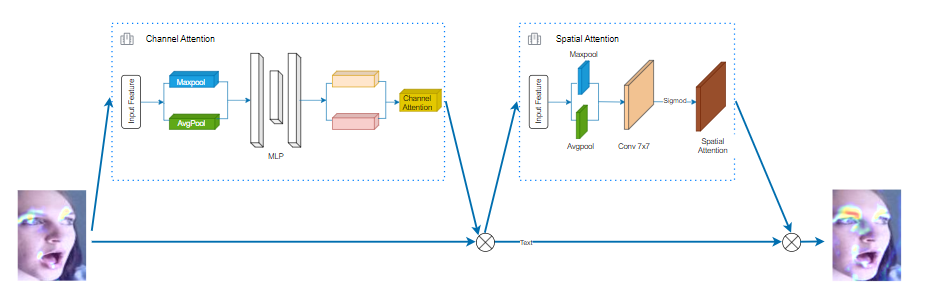
\includegraphics[width=0.9\textwidth]{Figures/CBAM.png}
   \caption{CBAM Attention Module}
  \label{fig:hinh-anh-6}
\end{figure}


\subsection{BAM - Bottleneck Attention Module}
BAM(Bottleneck Attention Module) \cite{b8} is an attention module that combines both channel attention and spatial attention in a sequential manner. It is designed to be lightweight and efficient, suitable for deep networks.

Channel Attention in BAM: Employs a sub-network with a bottleneck layer to reduce the channel dimensionality, followed by an up-projection to restore the original dimensionality. This process helps the network learn inter-channel relationships and generate weights for each channel. A sigmoid function is used to normalize these weights to the range (0, 1).
% \[
% M_c(X) = \sigma\left(\text{MLP}\left(\text{AvgPool}(X) + \text{MaxPool}(X)\right)\right)  
% \]
\begin{equation}\label{eq:cbam-channel}
M_c(X) = \sigma\bigl(\mathrm{MLP}(\mathrm{AvgPool}(X)) + \mathrm{MLP}(\mathrm{MaxPool}(X))\bigr)
\end{equation}
Spatial Attention in BAM: A convolutional layer is employed to generate a spatial attention map. This map indicates the importance of each spatial location. A sigmoid function is also utilized here.
% \[
% M_s(X) = \sigma\left(\text{ReLU}\left(\text{BatchNorm}\left(\text{Conv2D}(X)\right)\right)\right) 
% \]
\begin{equation}\label{eq:cbam-spatial}
M_s(X) = \sigma\Bigl(\mathrm{Conv2D}\bigl(\bigl[\mathrm{AvgPool}(X),\,\mathrm{MaxPool}(X)\bigr]\bigr)\Bigr)
\end{equation}
BAM combines the outputs of two branches, channel attention and spatial attention, which are multiplied element-wise and then added to the original input. This process helps the network enhance important features and mitigate the influence of less important ones.
% \[
% X_{\text{out}} = X \odot \left( M_c(X) + M_s(X) \right)
% \]
\begin{equation}\label{eq:cbam-out}
X_{\mathrm{out}} = X \odot M_c(X) \odot M_s(X)
\end{equation}
\begin{figure}[h]
  \centering
  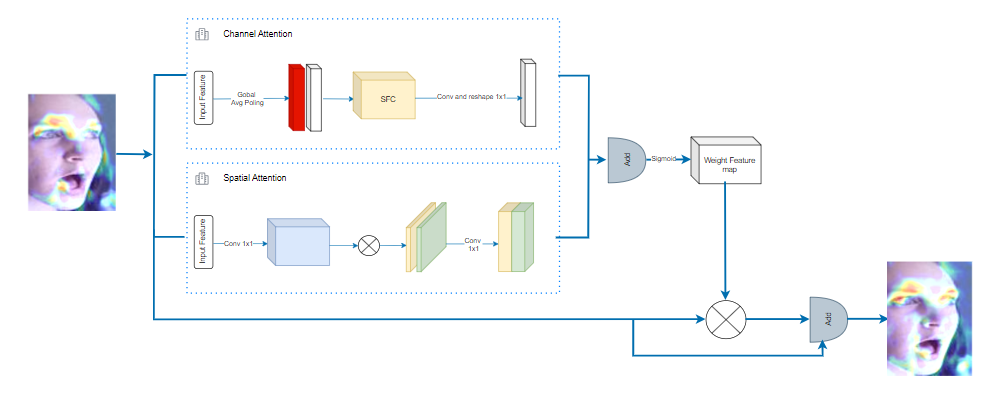
\includegraphics[width=0.9\textwidth]{Figures/BAM2.png}
   \caption{BAM Attention Module}
  \label{fig:hinh-anh-7}
\end{figure}

\subsection{scSE - spatial and channel Squeeze Excitation}
scSE (Spatial and channel Squeeze \& Excitation) \cite{b9} is a variant of SE (Squeeze \& Excitation) that incorporates both channel attention and spatial attention in a parallel manner.

\begin{figure}[h]
  \centering
  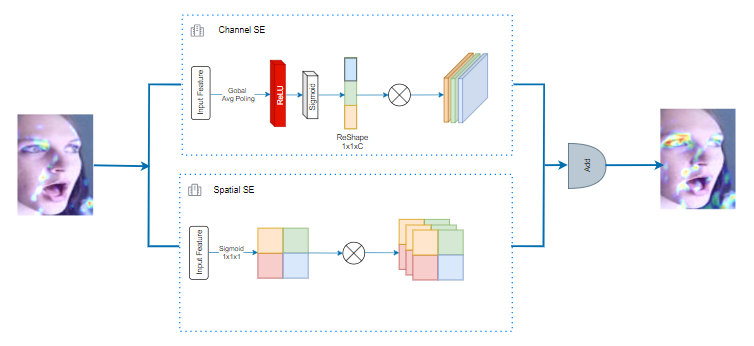
\includegraphics[width=0.7\textwidth]{Figures/scse2.png}
   \caption{Spatial Attention Module}
  \label{fig:hinh-anh-8}
\end{figure}
Channel Attention in scSE (cSE - channel SE): Similar to the original SE, it utilizes global average pooling to "squeeze" spatial information into a feature vector for each channel. Subsequently, a sub-network with two fully connected layers is employed to learn inter-channel relationships and generate weights.

% \[  
% M_C(X) = \sigma(\text{MLP}(\text{AvgPool}(X)))  
% \]  
\begin{equation}\label{eq:scse-channel}
M_{cSE}(X) = \sigma\bigl(\mathrm{MLP}(\mathrm{AvgPool}(X))\bigr)
\end{equation}
Spatial Attention in scSE (sSE - spatial SE): A 1x1 convolution is employed to reduce the channel dimensionality to 1, followed by the application of a sigmoid function to generate a spatial attention map.
\begin{equation}\label{eq:scse-spatial}
M_{sSE}(X) = \sigma\bigl(\mathrm{Conv}_{1\times1}(X)\bigr)
\end{equation}

scSE combines the two branches, cSE (channel Squeeze-and-Excitation) and sSE, via element-wise addition, which is then multiplied by the original input.
% \[ 
% X_out=X_cSE+X_sSE 
% \]  
\begin{equation}\label{eq:scse-out}
X_{\mathrm{out}} = X_{cSE} + X_{sSE}
\end{equation}
\section{The effectiveness of attention}\label{sec3}
\subsection{Integration with the CNN}


\begin{figure}[ht]  
    \centering  
    \begin{minipage}{0.6\textwidth}  
        \centering  
        % Include the figure  
        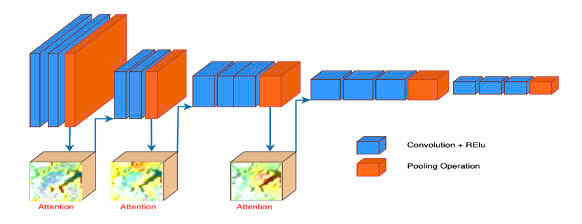
\includegraphics[width=\textwidth]{Figures/vgg_config.jpg}  
        \caption{VGGNet with Attention Configuration}  
        \label{fig:hinh-anh-9}  
    \end{minipage}%  
    \begin{minipage}{0.4\textwidth}  
        \centering  
        \small % or \footnotesize or \scriptsize 
        \begin{tabular}{@{}ll@{}}  
            \toprule  
            \textbf{Layer Name} & \textbf{Configuration} \\ \midrule  
            Conv Block 1 & [3x3, 64] x2 \\
            & MaxPooling \\ \midrule  
            Conv Block 2 & [3x3, 128] x2 \\
            & MaxPooling \\ \midrule  
            Conv Block 3 & [3x3, 256] x3 \\
            & MaxPooling \\ \midrule  
            Conv Block 4 & [3x3, 512] x3 \\
            & MaxPooling \\ \midrule  
            Conv Block 5 & [3x3, 512] x3 \\
            & MaxPooling \\ \midrule  
            FC Layers & FC-2048 \\ \midrule  
            Output & FC-7 \\
            & Soft-Max \\ \bottomrule  
        \end{tabular}  
        \caption{VGG16 Architecture}  
    \end{minipage}  
\end{figure} 
\textbf{VGG16:} The image is passed through a series of convolutional layers with a kernel size of (3x3). This kernel size is the smallest size that can easily identify left-right, up-down, and center positions. The convolution stride is fixed at 1, and padding is set to "same" to preserve the spatial resolution after convolution. Max-pooling is applied with a stride of two after a certain number of convolutions to reduce the output size of the convolutional layer. Here, the output feature map of the pooling serves as the input to the Attention Module.

Finally, a series of convolutional layers (with varying depths across different architectures) is followed by three fully connected layers: the first two layers have 2048 channels each, and the third layer contains seven channels (one for each class). The final layer is a soft-max layer and computes the output emotion class.

\begin{figure}[ht]  
    \centering  
    \begin{minipage}{0.6\textwidth}  
        \centering  
        % Include the figure (replace with your actual image path)  
        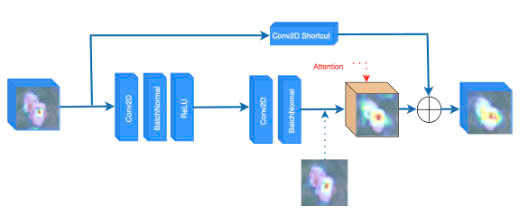
\includegraphics[width=\textwidth]{Figures/residual_config.jpg}  
        \caption{Attention configuration within the Residual block}  
        \label{fig:hinh-anh-resnet18}  
    \end{minipage}%  
    \begin{minipage}{0.3\textwidth}  
        \centering  
        
        \small
        % Change font size for the table  
        \small % or \footnotesize or \scriptsize  
        \begin{tabular}{@{}ll@{}}  
            \toprule  
            \textbf{Layer Name} & \textbf{Configuration} \\ \midrule  
            Conv Block 1 & Conv 7x7, 64, Stride 2 \\
            & 3 x 3 MaxPool, Stride 2 \\ \midrule  
            Conv Block 2 &   
            \(\left[\begin{array}{cc}  
            1 \times 1, & 64 \\
            3 \times 3, & 64 \\
            1 \times 1, & 256  
            \end{array}\right] \times 2\) \\ \midrule  
            Conv Block 3 &   
            \(\left[\begin{array}{cc}  
            1 \times 1, & 64 \\
            3 \times 3, & 64 \\
            1 \times 1, & 256  
            \end{array}\right] \times 2\) \\ \midrule  
            Conv Block 4 &   
            \(\left[\begin{array}{cc}  
            1 \times 1, & 64 \\
            3 \times 3, & 64 \\
            1 \times 1, & 256  
            \end{array}\right] \times 2\) \\ \midrule   
            Conv Block 5 &   
            \(\left[\begin{array}{cc}  
            1 \times 1, & 64 \\
            3 \times 3, & 64 \\
            1 \times 1, & 256  
            \end{array}\right] \times 2\) \\ \bottomrule  
        \end{tabular}  
        \caption{ResNet 18 Architecture}  
    \end{minipage}  
\end{figure} 

\textbf{ResNet18:} While ResNet is a more complex architecture, the optimal approach to integrate Attention is within the residual block. This integration can be seen in Figure 11, which illustrates the Attention module diagram for ResNet. The attention module is added before the element-wise addition with the identity branch. ECA-Net\cite{b13} and the attention mechanisms we use also follow the same integration strategy with the Residual block.




\subsection{Dataset}

Experiments were conducted on the RAF-DB, FER-2013, and CIFAR-10 datasets using ResNet18 and VGG16 architectures.
\begin{figure}[h]  
    \centering  
    \begin{subfigure}{0.3\textwidth}  
        \centering  
        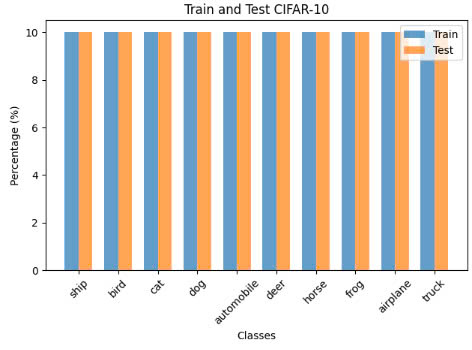
\includegraphics[width=\linewidth]{Figures/CIFA_Distribution.jpg}
        \caption{CIFAR-10}  
        \label{fig:cifar-distribution}  
    \end{subfigure}  
    \hfill  
    \begin{subfigure}{0.3\textwidth}  
        \centering  
        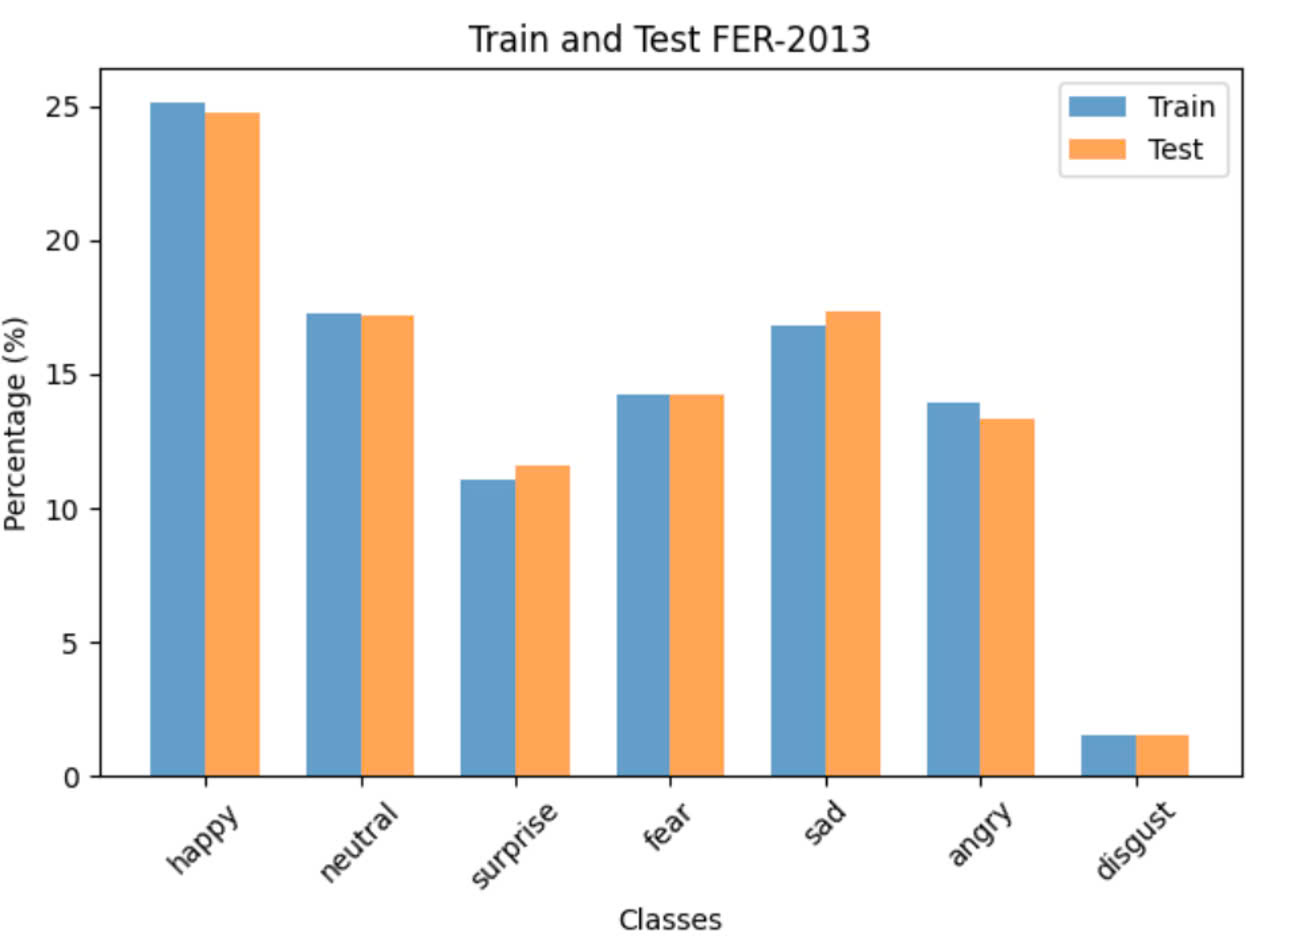
\includegraphics[width=\linewidth]{Figures/FER_Distribution.jpg}
        \caption{FER-2013}  
        \label{fig:fer-distribution}  
    \end{subfigure}  
    \hfill  
    \begin{subfigure}{0.3\textwidth}  
        \centering  
        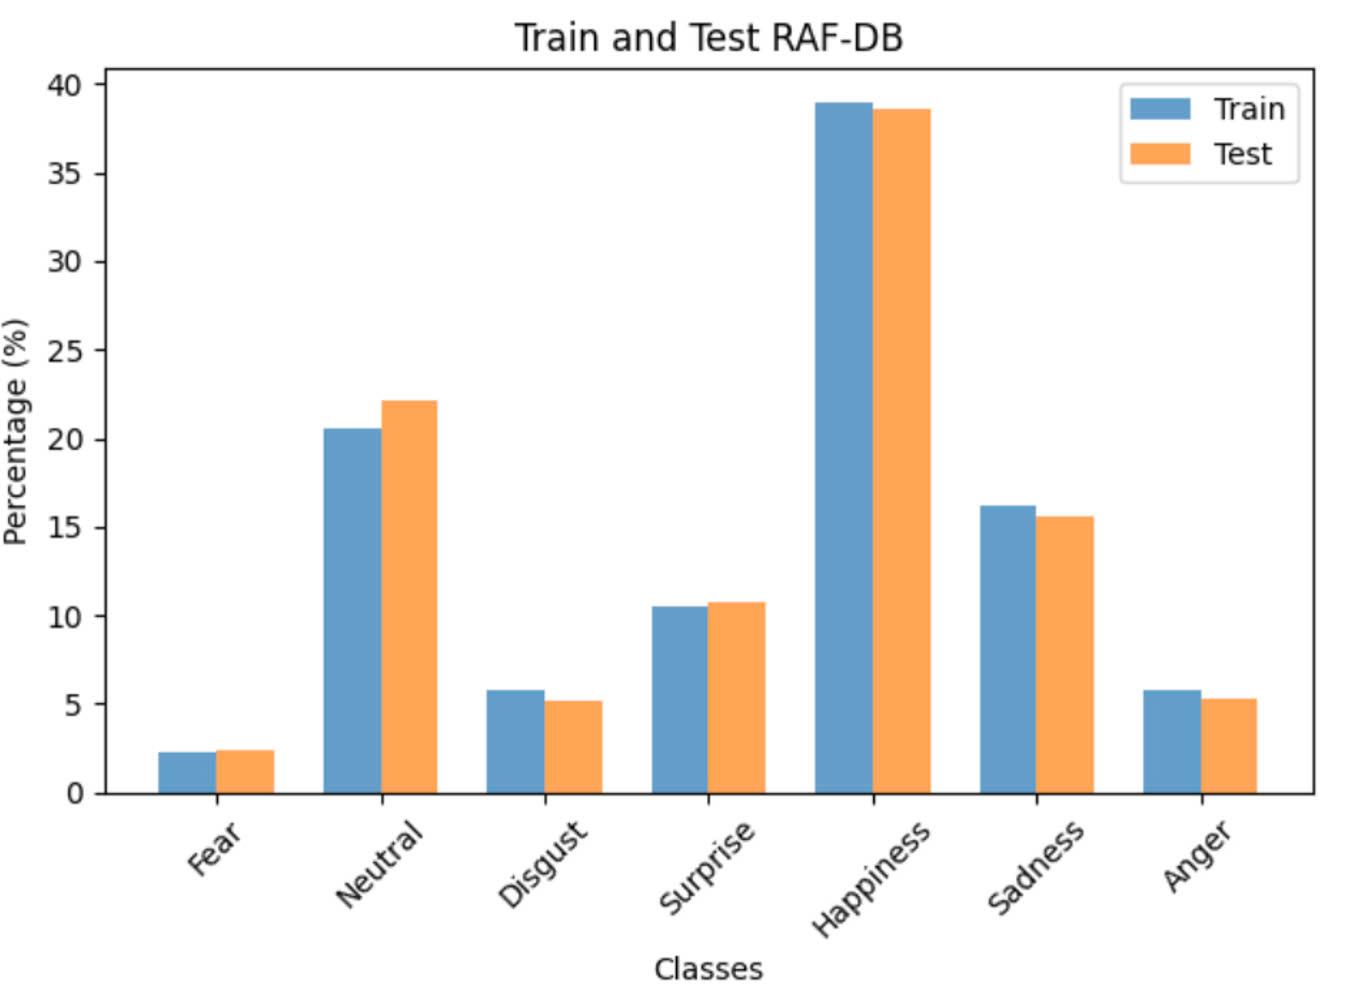
\includegraphics[width=\linewidth]{Figures/RAFDB_Distribution.jpg}
        \caption{RAF-DB}  
        \label{fig:rafdb-distribution}  
    \end{subfigure}  
    \caption{Ratio of labels in datasets}  
    \label{fig:cifar-group}  
\end{figure}  
Fig.a RAF-DB is a widely-used dataset designed for real-world facial emotion recognition, comprising 15,339 images, of which 12,271 are designated for training (approximately 80\%) and 3,068 for testing (approximately 20\%). Fig.b FER2013 is a popular dataset in the field of emotion recognition, consisting of 35,887 grayscale images, each with a fixed size of 48x48 pixels. Specifically, the training set contains 28,709 images, and the test set contains 7,178 images. The facial images depict various emotional states corresponding to seven emotion labels ("angry", "disgust", "fear", "happy", "neutral", "sad", "surprise"). Fig.c CIFAR-10 (Canadian Institute for Advanced Research) is a well-known dataset in the computer vision domain introduced by Alex Krizhevsky, Geoffrey Hinton, and Vinod Nair, comprising 60,000 color images, with 50,000 images in the training set and 10,000 images in the test set. The image dimensions are 32x32 pixels. CIFAR-10 consists of 10 classes with a balanced number of images per class.


\subsection{Experimental process}

Input images were resized to 224×224×3 for RAF-DB, 48x48x1 for FER-2013, and 32x32x3 for CIFAR-10. We employed ImageDataGenerator to generate image augmentations during training. The augmentations we applied included random rotations between -20 and +20 degrees, horizontal and vertical shifts, and zoom/range zooming with a ratio of 20\%. Labels were converted to one-hot encoding. The number of epochs was limited to 120.

We trained the model using the Adam optimizer, with an initial learning rate of 0.0001. The learning rate schedule was ExponentialDecay, with a minimum learning rate of 0.00001. Each experiment utilized an early stopping method with a patience of 50 epochs and saved weights only when the highest validation accuracy was achieved. The training/testing split ratio was 80/20\%. Experiments were conducted on a virtual machine with an NVIDIA Tesla P100 GPU. Other parameters are detailed in Table 1.

\begin{table}[ht]
    \centering
    \caption{Experimental process}
    \label{tab1}
    \begin{tabular}{|c|c|c|c|}
    \hline
    \textbf{} & \textbf{Calibration Parameters} & \textbf{Search Space} & \textbf{Final Settings}  \\
    \hline
    & Learning Rate & 0.1, 0.001, 0.0001, 0.00001 & 0.0001 \\
    & Batch Size RAF-DB	 & 6, 32, 64, 32 & 32 \\
    & Batch Size CIFA & 32, 64, 128, 256 & 128 \\
    & Batch Size FER & 32, 64, 128, 256 & 64 \\
    & Activation Functions & ReLU, ELU, SELU & ELU \\
    & Optimizer & Adam, sgd, rmsprop, adadelta, adamax & Adam \\
    & Pooling & Max Pooling, Average Pooling & Average Pooling \\
    & CBAM Reduction Ratio & 4, 8, 16, 32 & 16 \\
    & BAM Reduction Ratio & 4, 8, 16, 32 & 16 \\
    & SCSE Reduction Ratio & 4, 8, 16, 32 & 16 \\
    \hline
    \end{tabular}
\end{table}
\begin{table}[ht]
    \centering
    \caption{Baseline models without attention (ResNet18 and VGG16)}
    \label{tab1}
    \begin{tabular}{|c|c|c|c|c|c|}
    \hline
    \textbf{} & \textbf{Model} & \textbf{Param (M)} & \textbf{RAF-DB} & \textbf{FER-2013}  & \textbf{CIFA-10}\\
    \hline
    & VGG16 & 15.77 & 81.13\% & 67.99\% & 84\% \\
    & ResNet18 & 13.95 &  81.81\% & 61.84\% & 86.69\% \\
    \hline
    \end{tabular}
\end{table}
\begin{table}[ht]
    \centering
    \caption{ResNet18 and VGGNet16 combined with Attentions on all Stage}
    \label{tab2}
    \begin{tabular}{|c|c|c|c|c|c|}
    \hline
    \textbf{} & \textbf{Model} & \textbf{Param (M)} & \textbf{RAF-DB} & \textbf{FER-2013}  & \textbf{CIFA-10}\\
    \hline
    & VGG16 + CBAM + full & 15.77 & 80.21\% & 68.07\% & 86.77\% \\
    & VGG16 + BAM + full & 17.00 & \textbf{82.63\%(1.5\%)} & 68.11\% & 84.44\% \\
    & VGG16 + SCSE + full & 16.92 & 81.84\% & 67.94\% & 84.09\% \\
    & ResNet-18 + CBAM + full & 16.10 & 80.22\% & \textbf{65.03\%(3.19\%)}  & \textbf{89.06\%(5.06\%) } \\
    & ResNet-18 + BAM + full & 16,86 & 80.15\% & 62.21\% & \textbf{87.92\%(1.23\%)} \\
    & ResNet-18 + SCSE + full & 16.92 & 80.05\% & 61.99\% & 87.11\% \\
    \hline
    \end{tabular}
\end{table}
\begin{table}[ht]
    \centering
    \caption{ResNet18 and VGGNet16 combined with Attentions on Stage 1,2,3}
    \label{tab3}
    \begin{tabular}{|c|c|c|c|c|c|}
    \hline
    \textbf{} & \textbf{Model} & \textbf{Param (M)} & \textbf{RAF-DB} & \textbf{FER-2013}  & \textbf{CIFA-10}\\
    \hline
    & VGG16 + CBAM + s123 & 15.83 & \textbf{82.63\%(1.5\%)} & \textbf{69.62\%(1.63\%)} & 83.91\% \\
    & VGG16 + BAM + s123 & 15.80 & \textbf{83.83\%(2.7\%)} & 69.09\% & 84.37\% \\
    & VGG16 + SCSE + s123 & 15.79 & \textbf{84.19\%(3.06\%) }& \textbf{69.07\%(1.08\%)} & \textbf{86.73\%(2.73\%)} \\
    & ResNet-18 + CBAM + s123 & 14.65 & 76.17\% & \textbf{65.23\%(3.39\%)} & \textbf{89.06\%(5.06\%)} \\
    & ResNet-18 + BAM + s123 & 14.68 & 80.70\% & \textbf{67.33\%(5.49\%)} & 77.95\% \\
    & ResNet-18 + SCSE + s123 & 14.29 & 82.46\% & \textbf{67.34\%(5.5\%) }& \textbf{89.40\%(2.71\%)} \\
    \hline
    \end{tabular}
\end{table}

\newpages

\begin{figure}[h]
\centering
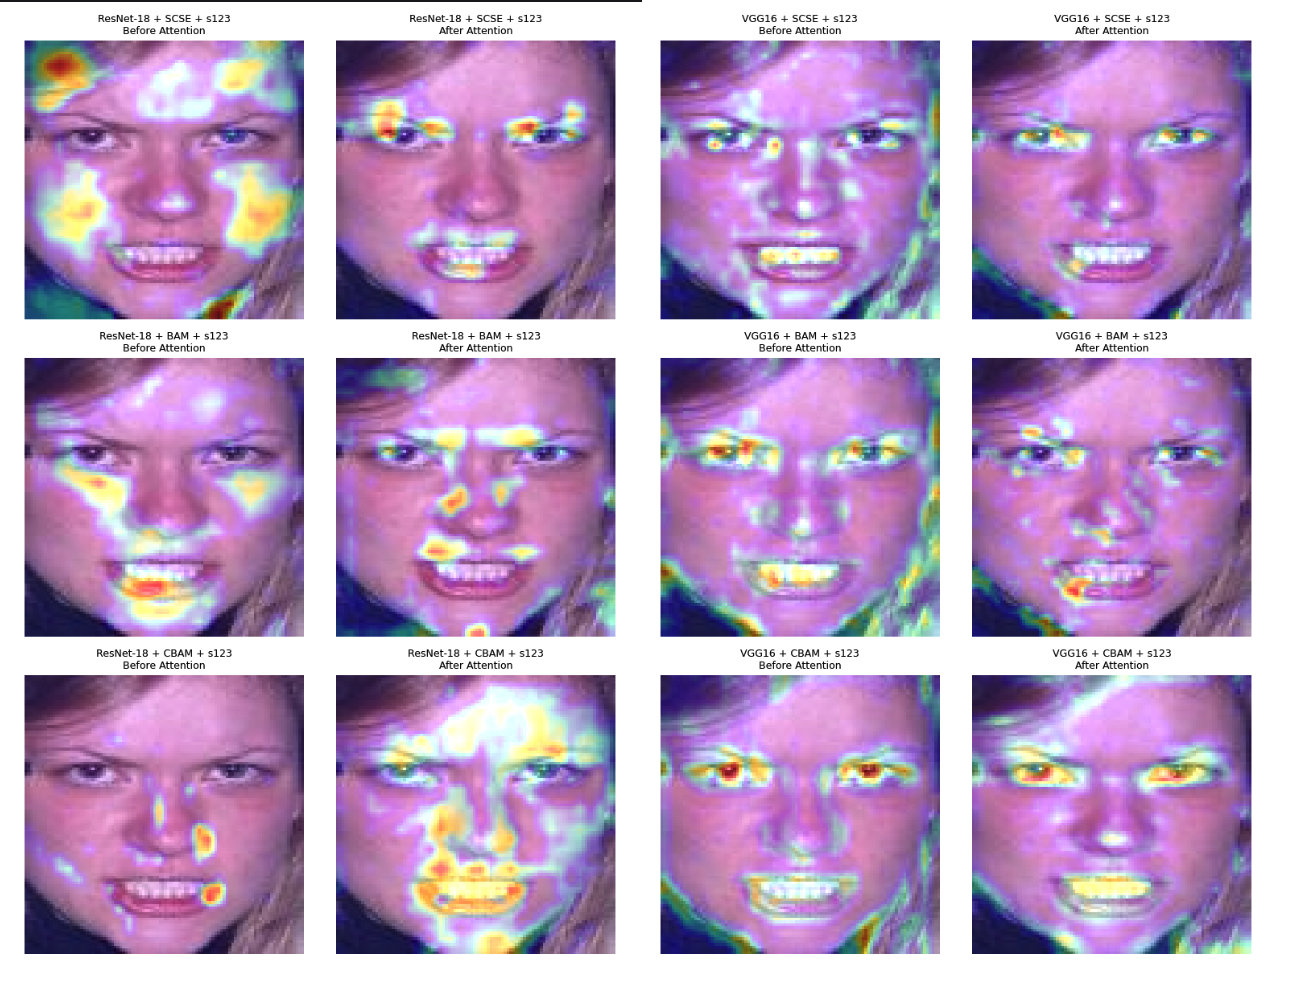
\includegraphics[width=0.8\textwidth]{Figures/grad-cam.png}
\caption{
The Grad-CAM image illustrates the distribution of model activations before and after applying the SCSE, BAM, and CBAM attention modules on ResNet-18 and VGG16 architectures, using the RAF-DB dataset. Before attention is applied, activations are scattered across irrelevant regions such as the background and non-facial areas.
}
\label{fig:gradcam}
\end{figure}

\subsection{Results and discussion}
We conducted experiments on training conventional networks. The results are presented in Table 2. The best accuracy scores were achieved by both ResNet and VGG models, with accuracy values of 86.69\% and 84\% on the CIFAR-10 dataset, respectively. We attached the Attention module to the first three Stages in each Residual block of the ResNet network and the first three Convolution Blocks of the VGG network simultaneously, and also attached it to all Stages as well as all Blocks of the two networks. The performance of ResNet and VGG with Attention at all stages was almost identical to the model without Attention and even showed some performance degradation. Conversely, attaching Attention to the first three stages significantly increased the accuracy score across all Attention modules. The results from the study ruled out attaching Attention at all stages. Our experimental results, presented in Table 3, show that Attention at the first three stages helps extract features more effectively than at all stages, with a score improvement from the scSE module of 3\% on the RAF-DB dataset, 1\% on the FER-2013 dataset, and 2\% on CIFAR-10. However, when Attention was used at all stages, the performance did not improve compared to Attention used only at the first three stages. This concludes that the first two or three stages play a crucial role in generating more effective refined feature maps compared to deeper stages. This is because these feature maps have already achieved a certain level of convergence when the CNN model learns too deeply, leading to the extraction of information from the two spatial domains no longer being effective. However, from Table 3, we observe that the results are still good and show signs of increased accuracy on the CIFAR-10 and FER datasets for the scSE module. This demonstrates that modules developed later, such as scSE, can still extract features at later stages after the model has learned deeper.


\section{Conclusion}\label{secA1}

In this study, we investigated the effectiveness of integrating attention mechanisms—CBAM, BAM, and scSE—into ResNet18 and VGG16 architectures for enhancing image classification performance across multiple datasets, including RAF-DB, FER-2013, and CIFAR-10. Through extensive experimentation, we observed that inserting attention modules into the early stages of the network (Stages 1–3) consistently yields higher accuracy compared to applying attention throughout the network.

Among the tested mechanisms, scSE, which combines both spatial and channel attention in parallel, demonstrated superior performance across most datasets. This confirms the hypothesis that early feature maps in CNNs carry critical information and are more sensitive to selective enhancement via attention.

However, while performance gains are evident, the inclusion of attention mechanisms introduces additional computational overhead. This trade-off highlights the importance of selective and efficient attention integration, especially for deployment in resource-constrained environments.

Future work should focus on:

Performing detailed computational cost analysis (e.g., FLOPs, parameter count, and inference latency).

Exploring lightweight and adaptive attention modules such as ECA or SE-lite.

Investigating hybrid attention mechanisms in transformer-CNN fusion models for real-time applications.

%%=============================================%%
%% For submissions to Nature Portfolio Journals %%
%% please use the heading ``Extended Data''.   %%
%%=============================================%%

%%=============================================================%%
%% Sample for another appendix section			       %%
%%=============================================================%%

%% \section{Example of another appendix section}\label{secA2}%
%% Appendices may be used for helpful, supporting or essential material that would otherwise 
%% clutter, break up or be distracting to the text. Appendices can consist of sections, figures, 
%% tables and equations etc.


%%===========================================================================================%%
%% If you are submitting to one of the Nature Portfolio journals, using the eJP submission   %%
%% system, please include the references within the manuscript file itself. You may do this  %%
%% by copying the reference list from your .bbl file, paste it into the main manuscript .tex %%
%% file, and delete the associated \verb+\bibliography+ commands.                            %%
%%===========================================================================================%%



% \begin{thebibliography}{99}
% \bibitem{ref1} K. O’Shea and R. Nash, "An introduction to convolutional neural networks," no. ArXiv Prepr. ArXiv151108458, 2015.
% \bibitem{ref2} Y. LeCun, L. Bottou, Y. Bengio and P. Haffner, “Gradient-based learning,” vol. 86, IEEE, 1998, p. 2278–2324.
% \bibitem{ref3} K. Simonyan and A. Zisserman, "Very Deep Convolutional Networks for," 2015.
% \bibitem{ref4} K. He and X. Zhang, "Deep Residual Learning for Image Recognition," in Proceedings of the IEEE Conference on Computer Vision and Pattern Recognition (CVPR), Las Vegas, NV, USA, pp. 770–778, 2015.
% \bibitem{ref5} S. Woo, J. Park, J.-Y. Lee, and I. S. Kweon, "CBAM: Convolutional Block Attention Module," in Proceedings of the European Conference on Computer Vision (ECCV), Munich, Germany, pp. 3–19, 2018.
% \bibitem{ref6} Z. Yu and C. Zhang, "Image-based Static Facial Expression Recognition with Multiple Deep Network Learning," in Proceedings of the IEEE Conference on Computer Vision and Pattern Recognition Workshops (CVPRW), Boston, MA, USA, pp. 94–101, 2015.
% \bibitem{ref7} C. Pramerdorfer and M. Kampel, "Facial Expression Recognition using Convolutional Neural Networks: State of the Art," Journal of Image and Vision Computing, vol. 54, pp. 123–134, 2016.
% \bibitem{ref8} R. Breuer and R. Kimmel, "A Deep Learning Perspective on the Origin of Facial Expressions," Nature Communications, vol. 8, pp. 564–576, 2017.
% \bibitem{ref9} S. Li and W. Deng, "Reliable Crowdsourcing and Deep Locality-Preserving Learning for Unconstrained Facial Expression Recognition," IEEE Transactions on Image Processing, vol. 27, no. 1, pp. 97–108, 2018.
% \bibitem{ref10} Y. Wang, Y. Li, Y. Song, and X. Rong, "Facial Expression Recognition Based on Auxiliary Models," in Proceedings of the IEEE International Conference on Pattern Recognition (ICPR), Beijing, China, pp. 421–430, 2019.
% \bibitem{ref11} D. Kollia and S. Zafeirriou, "Expression, Affect, Action Unit Recognition: Aff-Wild2, Multi-Task Learning and ArcFace," in Proceedings of the IEEE International Conference on Computer Vision (ICCV), Seoul, South Korea, pp. 2342–2351, 2019.
% \bibitem{ref12} M.-I. Georgescu, R. T. Iones, and M. Popescu, "Local Learning with Deep and Handcrafted Features for Facial Expression Recognition," Pattern Recognition Letters, vol. 133, pp. 15–25, 2020.
% \bibitem{ref13} T. H. Vo, G.-S. Lee, H.-J. Yang, and S.-H. Kim, "Pyramid With Super Resolution for In-The-Wild Facial Expression Recognition," IEEE Access, vol. 8, pp. 219–232, 2020.
% \bibitem{ref14} J. L. Joseph and S. P. Mathew, "Facial expression recognition for the blind using deep learning," Expert Systems with Applications, vol. 176, pp. 1–10, 2021.
% \bibitem{ref15} D. Kollias, V. Sharmanska, and S. Zafeiriou, "Distribution Matching for Heterogeneous Multi-Task Learning: a Large-scale Face Study," Neural Networks Journal, vol. 142, pp. 125–137, 2021.
% \bibitem{ref16} O. C. Oguine, K. J. Oguine, H. I. Bisallah, and D. Ofuani, "Hybrid Facial Expression Recognition (FER2013) Model for Real-Time Emotion Classification and Prediction," Applied Sciences, vol. 12, pp. 423–439, 2022.
% \bibitem{ref17} Y. Zhang, C. Wang, X. Ling, and W. Deng, "Learn From All: Erasing Attention Consistency for Noisy Label Facial Expression Recognition," IEEE Transactions on Neural Networks and Learning Systems, vol. 34, no. 5, pp. 674–687, 2022.
% \bibitem{ref18} G. I. Tutuianu, Y. Liu, A. Alamäki, and J. Kauttonen, "Benchmarking Deep Facial Expression Recognition: An Extensive Protocol with Balanced Dataset in the Wild," Journal of Machine Vision and Applications, vol. 34, pp. 567–578, 2023.
% \bibitem{ref19}Simonyan, K. and Zisserman, A. 2014. Very Deep Convolutional Networks for LargeScale Image Recognition. 3rd International Conference on Learning
% Representations, ICLR 2015 - Conference Track Proceedings
% \bibitem{ref20}Woo, S., Park, J., Lee, J.Y. and Kweon, I.S. 2018. CBAM: Convolutional block
% attention module In: Lecture Notes in Computer Science (including subseries
% Lecture Notes in Artificial Intelligence and Lecture Notes in Bioinformatics)
% [Online]. Springer Verlag, pp.3–19. [Accessed 14 April 2022]. Available from:
% https://link.springer.com/chapter/10.1007/978-3-030-01234-2\_1.
% \bibitem{ref21}J. Park, S. Woo, J.-Y. Lee, and I. S. Kweon, “Bam: Bottleneck
% attention module,” 2018.
% \bibitem{ref22}A. G. Roy, N. Navab, and C. Wachinger, “Recalibrating fully
% convolutional networks with spatial and channel “squeeze and
% excitation” blocks,” IEEE transactions on medical imaging, vol. 38,
% no. 2, pp. 540–549, 2018.
% \bibitem{ref23}Wang, Q., Wu, B., Zhu, P., Li, P., Zuo, W. and Hu, Q. 2020. ECA-Net: Efficient
% channel attention for deep convolutional neural networks. Proceedings of the
% IEEE Computer Society Conference on Computer Vision and Pattern
% Recognition., pp.11531–11539.
% \end{thebibliography}


\printbibliography
\end{document}
